% !TeX spellcheck = de_DE
\section{Finite Elemente Methode}
	
	\subsection{Angabe}
	Es soll die Methode der finiten Elemente (FEM) auf folgende Gleichung angewendet werden.
	\begin{equation}
		\frac{\partial^2 u(x,t)}{\partial ^2 x} - \mu_0 \epsilon_0 \frac{\partial ^2 u (x,t)}{\partial^2 t} = 0
	\end{equation}
	Mit den Randbedingungen
	\begin{align}
	u(a,t) &= 0 \\
	- \frac{\partial}{\partial x} u(b,t)+\sqrt{\mu_0 \epsilon_0} \frac{\partial}{\partial t} u(b,t) &= 0
	\end{align}
	Mit den Anfangsbedingungen
	\begin{align}
	u(x,0) &= w(x) = e^{-k(2x-a-b)^2} \\
	\frac{\partial}{\partial t} u(x,0) &= 0
	\end{align}
	soll das Newmarksche Zeitschrittverfahren durchgeführt werden.
	\\
	
	{\Large Aufgaben \par}
	\begin{enumerate}
		\item Leiten Sie dazu die schwache Formulierung für die Abhängigkeit vom Ort her.
		\item Nehmen Sie eine geeignete Länge des Intervalls $[a, b]$ an und unterteilen Sie es gleichmäßig in $n$ finite Elemente der Länge $h$.
		\item Verwenden Sie Hutfunktionen als Basisfunktionen. Berücksichtigen Sie die Randbedingungen und erstellen Sie die Steifigkeitsmarix $\mathbf{S}_h$ und die Massenmatrix $\mathbf{M}_h$.
		\item Lösen Sie das gewöhnliche Differentialgleichungssystem
	\[
	\mathbf{S}_h \mathbf{u}_h  + \mathbf{M}_h \frac{\partial ^2}{\partial t^2} \mathbf{u}_h = \mathbf{0}
	\]
		mit dem Newmark-Zeitschritt-Verfahren
	\end{enumerate}


	
	\subsection{Herleiten der schwachen Formulierung}
	\subsubsection{Allgemeine Idee}
	Wir betrachten Differentialgleichungssysteme auf einem Gebiet $\Omega$ (etwa ein Teil der reellen Zahlen $\mathbb{R}$) mit vorgegeben Werten (Randbedingungen) an $\partial \Omega$ die sich der Art 
	\begin{equation}
		\mathbf{A}\mathbf{u}=\mathbf{f}
	\end{equation}
	anschreiben lassen. Dabei ist $\mathbf{u}$ die gesuchte Funktion. Alle Faktoren und Differentialoperatoren werden durch $\mathbf{A}$ ausgedrückt. 
	Die Idee ist nun u durch eine Ansatzfunktion $u_h$ zu approximieren.
	Diese Ansatzfunktion soll in etwa die Gestalt einer Summe von (Laplace'schen) Ansatzfunktion multipliziert mit einem Trägerfunktion $p_i(x)$ sein. Diese Trägerfunktion soll im gesamten Gebiet mit Ausnahme eines kleinen Bereichs (eines \textit{Trägers}) verschwinden, also konstant 0 sein. Dadurch teilt man 
	\begin{equation}
		u_h = \sum_{i=0}^N u_i p_i(x)
	\end{equation}
	Diese Ansatzfunktion verändert unsere Funktion $u$, deshalb wird sie im Allgemeinen die Gleichung \textbf{nicht} erfüllen. Der linke Teil der Gleichung minus dem rechten Teil wird nicht exakt 0 sondern ein gewissen Wert $r$ ergeben. Dieser Fehler $r(x)$ wird \textit{Residuum} gennant.
	\begin{equation}
	\mathbf{r} =\mathbf{f}-\mathbf{A}\mathbf{u}_h \neq 0 \tag{allgemein}
	\end{equation}
	und in unserem Beispiel
	\begin{equation}
		r(x) =\frac{\partial^2 u_h(x,t)}{\partial ^2 x} - \mu_0 \epsilon_0 \frac{\partial ^2 u_h (x,t)}{\partial^2 t} \neq 0 
	\end{equation}
	Der tatsächliche Fehler (also der Differenz  $e=u-u_h$) kann, im Gegensatz zum Residuum, nicht bestimmt werden, da die Funktion $u$ nicht bekannt ist. Das Residuum kann jedoch bestimmt werden und dieses gilt es zu minimieren. Gesucht ist nun also:
	\begin{equation}
		\min{\mathbf{r}} = \min{\mathbf{f}-\mathbf{A}\mathbf{u}_h} =  0  \tag{hoffentlich}
	\end{equation}
	Bisher war es die Aufgabe die Funktion $u_h$ zu finden ($A$ und $f$ sind ja bekannt), welche die Residuuen verschwinden lässt. Wenn $u_h$
	Dazu wählen wir für die schwache Formulierung eine bekannte Gewichtsfunktion $w(x)$ und multiplizieren damit unsere Gleichung (\textit{Methode der gewichteten Residuuen}). Anschließend integrieren wir über das gesamte Gebiet $\Omega$ (was in unserem eindimensionalen Fall dem Intervall $[a,b]$ entspricht). Damit ergibt sich: 
	\begin{align}
	\int_{\Omega} r(x)w(x) dx = 0 \\
	\int_{a}^{b} u_h''(x,t) w(x) dx - \mu_0 \epsilon_0 \int_{a}^{b}\frac{\partial ^2 }{\partial t^2}u_h (x,t)w(x) dx =0 
	\label{weak-form}
	\end{align}
	Mit der verallgemeinerten Ableitung der Distributionen in $H$ (dem Sobolev-Raum, welcher Funktionen, für die eine verallgemeinerte Ableitung existiert umfasst):
	\begin{equation}
		\int_{a}^{b} u_h''(x) w(x) dx = -\int_{a}^{b} u_h'(x) w'(x) dx + u_h'(x)w(x) \vert_a^b 
		\label{distribution-differential}
	\end{equation}
	An $x=a$ (allgemeiner $\Gamma_D = \{a\}$) liegt eine Dirichlet'sche Randbedingung vor, was so viel bedeutet wie das $u(a,t)=\text{const}$ ist, damit muss die Weg-Ableitung $u'(a,t)$ verschwinden. Generell gilt hier, dass durch das Einsetzen der Ansatzfunktionen N Gleichungen erzeugt werden. Da der wert von $u$ an der Stelle $\Gamma_D = \{a\}$ allerdings bereits bekannt ist, wird diese Gleichung nicht benötigt damit kann $w(a)=0$ gewählt werden. Außerdem ist in unserem konkreten Fall noch eine Cauchy'sche Randbedingung an $\Gamma_C = \{b\}$ vorgegeben: 
	\[u'(b,t)=u_x(b,t) = \sqrt{\mu_0 \epsilon_0} u_t(b,t) ~~~~ \forall t \in  [0,t_0]\] daraus folgt also
	\begin{equation}
		u'(x,t)w(x) \vert_a^b = \sqrt{\mu_0 \epsilon_0} u_t (b,t) w(b) - \underbrace{u'(a,t)w(a)}_{=0}
	\end{equation}
	
	\subsection{Festlegen des Intervalls}
	Bei der Methode der finiten Elemente wird eine stetige Funktion auf $N$ Teilintervalle (Elemente) zerlegt. Dazu werden Funktionswerte an Knotenpunkten berechnet und diese mit auf kleine Intervalle beschränkten Funktionen multipliziert. Für das Intervall $x = \{a,...,b\}$ kann die Zerlegung folgendermaßen aussehen:
	\begin{equation}
	x_i = a + i h
	\end{equation}
	wobei die Schrittweite $h=\frac{b-a}{N}$ ist. Im Prinzip kann diese Zerlegung aber beliebig gewählt werden.
	\subsection{Ansatzfunktion}
	Für die Funktion $u$ wird eine Interpolation $u_h$ folgender Gestalt gewählt:
	\begin{equation}
	u \approx u_h = \sum_{i = 0}^{N} u_i  p_i(x)
	\end{equation}
	Dies entspricht einer Summe von Ansatzfunktion gewichtet mit noch zu bestimmenden konstanten Faktoren $u_i$. Diese Ansatzfunktion können verschiedene Gestalten haben, sollten jedoch die Eigenschaft aufweisen einen kompakten Träger zu besitzen, d.h. $p_i(x) = 0$ für alle $x > a+ih$ und $x < a-ih$. Zwischen zwei Knotenpunkten ist der Wert der Funktion nicht bekannt und muss entsprechend interpoliert werden und da sich zwischen den Kontenpunkten mehrere Ansatzfunktionen i.A. überlagern, sollte darauf geachtet werden, dass die Summe immer gleich 1 ist, also
	\begin{equation}
	p(x) = \sum_{i=0}^{N} p_i(x) = 1 ~~\forall x \in [a,b] 
	\end{equation} 
	Da die Koeffizienten $u_i$ nun konstante Faktoren sind, wird die (Weg-)Ableitung auf $p(x)$) übertragen. Das bedeutet:
	\begin{equation}
	u_h'(x,t) = \sum_{i = 0}^{N} u_i  p_i'(x)
	\end{equation}
%	Setzen wir dies in die allgemeine Formel \ref{generic-linear-equation} ein, erhalten wir:
%	\begin{equation}
%	A(\sum_{i = 0}^{N} u_i  p_i(x))-f(x,t)  \overset{!}{=} 
%	 0
%	\end{equation}
	In diesem Beispiel wird als Ansatzfunktionen verschobene Dreckeisfunktionen ('Hutfunktionen') verwendet. Selbstverständlich muss bei der Auswahl darauf geachtet werden, dass die gewählte Ansatzfunktion hinreichend oft differenzierbar ist.

	\begin{figure}
		\centering
		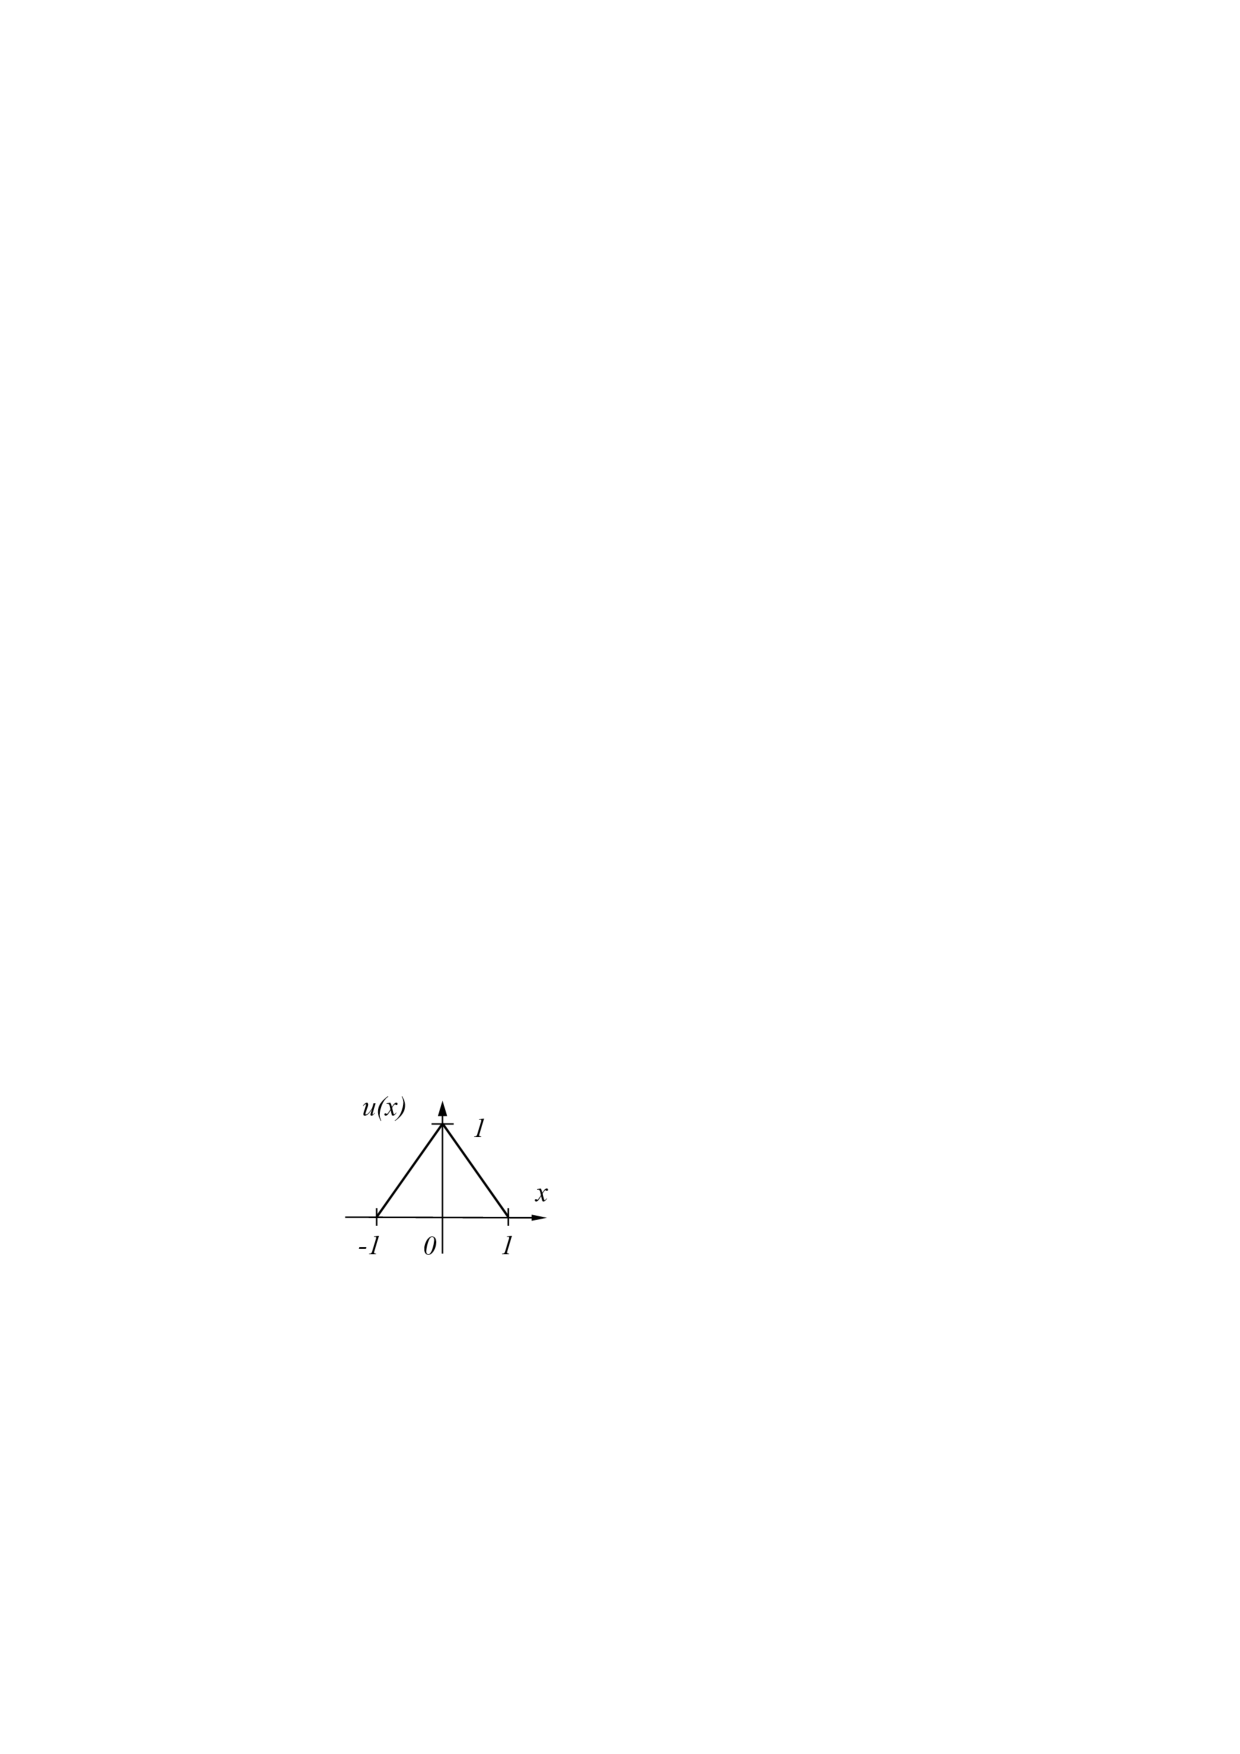
\includegraphics[width=0.5\linewidth]{img/hut}
		\caption[Hutfunktion]{Hutfunktion}
		\label{fig:hut}
	\end{figure}


	
	Setzen wir dies nun in die Herleitung der schwachen Formulierung \ref{weak-form} ein, erhalten wir mit etwas umformen und unter Verwendung der verallgemeinerten Ableitung aus Formel \ref{distribution-differential}. Da sich unser Intervall zeitlich nicht ändert, darf die Zeit-Ableitung vor das Integral gezogen werden.
	\begin{equation}
	\sum_{i = 0}^{N} u_i   \int_{a}^{b} p_i'(x) w'(x) dx - 
	\mu_0 \epsilon_0 \frac{\partial ^2 }{\partial t^2} \sum_{i = 0}^{N} u_i \int_{a}^{b}p_i(x)w(x) dx = 0
	\label{weak-form2}
	\end{equation}
	Hier gelten noch $u_1,u_2,...u_N$, also $N$ Unbekannte Koeffizienten, zu finden. Für $N$ unbekannte Koeffizienten werden bekanntlich $N$ unabhängige Gleichungen benötigt. Ein Weg diese zu erhalten ist über die Ansatzfunktion $v(x)$. Für diese Ansatzfunktion wird ebenfalls eine ähnliche Zerlegung wie für $p(x)$ festgelegt, sollte es sogar die selbe sein, handelt es sich um die \textit{Galerkin Methode}. Man setzt also
	\begin{equation}
	w(x) = p(x) = \sum_{j = 0}^{N} p_j(x)
	\end{equation}
	und setzt dies dann in die Gleichung (\ref{weak-form2}) ein.
	\begin{equation}
	\sum_{i = 0}^{N} u_i \sum_{j = 0}^{N}\int_{a}^{b} p_i' p_j' dx 
	+ 
	\sqrt{\mu \epsilon} \frac{\partial}{\partial t} u_i \sum_{j = 0}^{N} p_i(B) p_j
	= 
	\mu \epsilon \sum_{i = 0}^{N} \frac{\partial ^2 }{\partial t^2} u_i 
	\sum_{j = 0}^{N} \int_{a}^{b} p_i p_j dx
	\end{equation}
	
	Da wir Hutfunktionen verwenden können, welche durch die Dreiecksfunktion $p_i = tri(\frac{x + ih}{h})$ beschrieben werden, können die Integrale gelöst werden:
	
	\begin{equation}
	\int_{a}^{b} p_ip_j dx = \begin{cases}
	\frac{4}{6}h, ~~ j=i \\
	\frac{1}{6}h,~~ j=\{i-1,i+1\}\\
	0\, ~~\text{sonst}
	\end{cases}
	\end{equation}
	und für $p'_i p'_j$ gilt
	\begin{equation}
	\int_{a}^{b} p_i' p_j' dx = \begin{cases}
	\frac{2}{h}, ~~ j=i \\
	-\frac{1}{h},~~ j=\{i-1,i+1\}\\
	0\, ~~\text{sonst}
	\end{cases}
	\end{equation}
	Ausgenommen sind hier die Ergebnisse die direkt am Rand liegen. Bei $\Gamma_D = \{a\}$ ist der Wert von $u$ bereits bekannt, die Ansatzfunktion kann also ohne weiteres Null gesetzt werden. Bei $\Gamma_C = \{b\}$ ist nur der Wert der Ableitung von $u$ bekannt. Hier muss der Wert erst bestimmt werden. Bei Betrachtung der Situation am Rand sieht man, dass hier nur über die \textit{halbe} Ansatzfunktion integriert wird, also das auch genau halb so groß ist.
	\begin{figure}
		\centering
		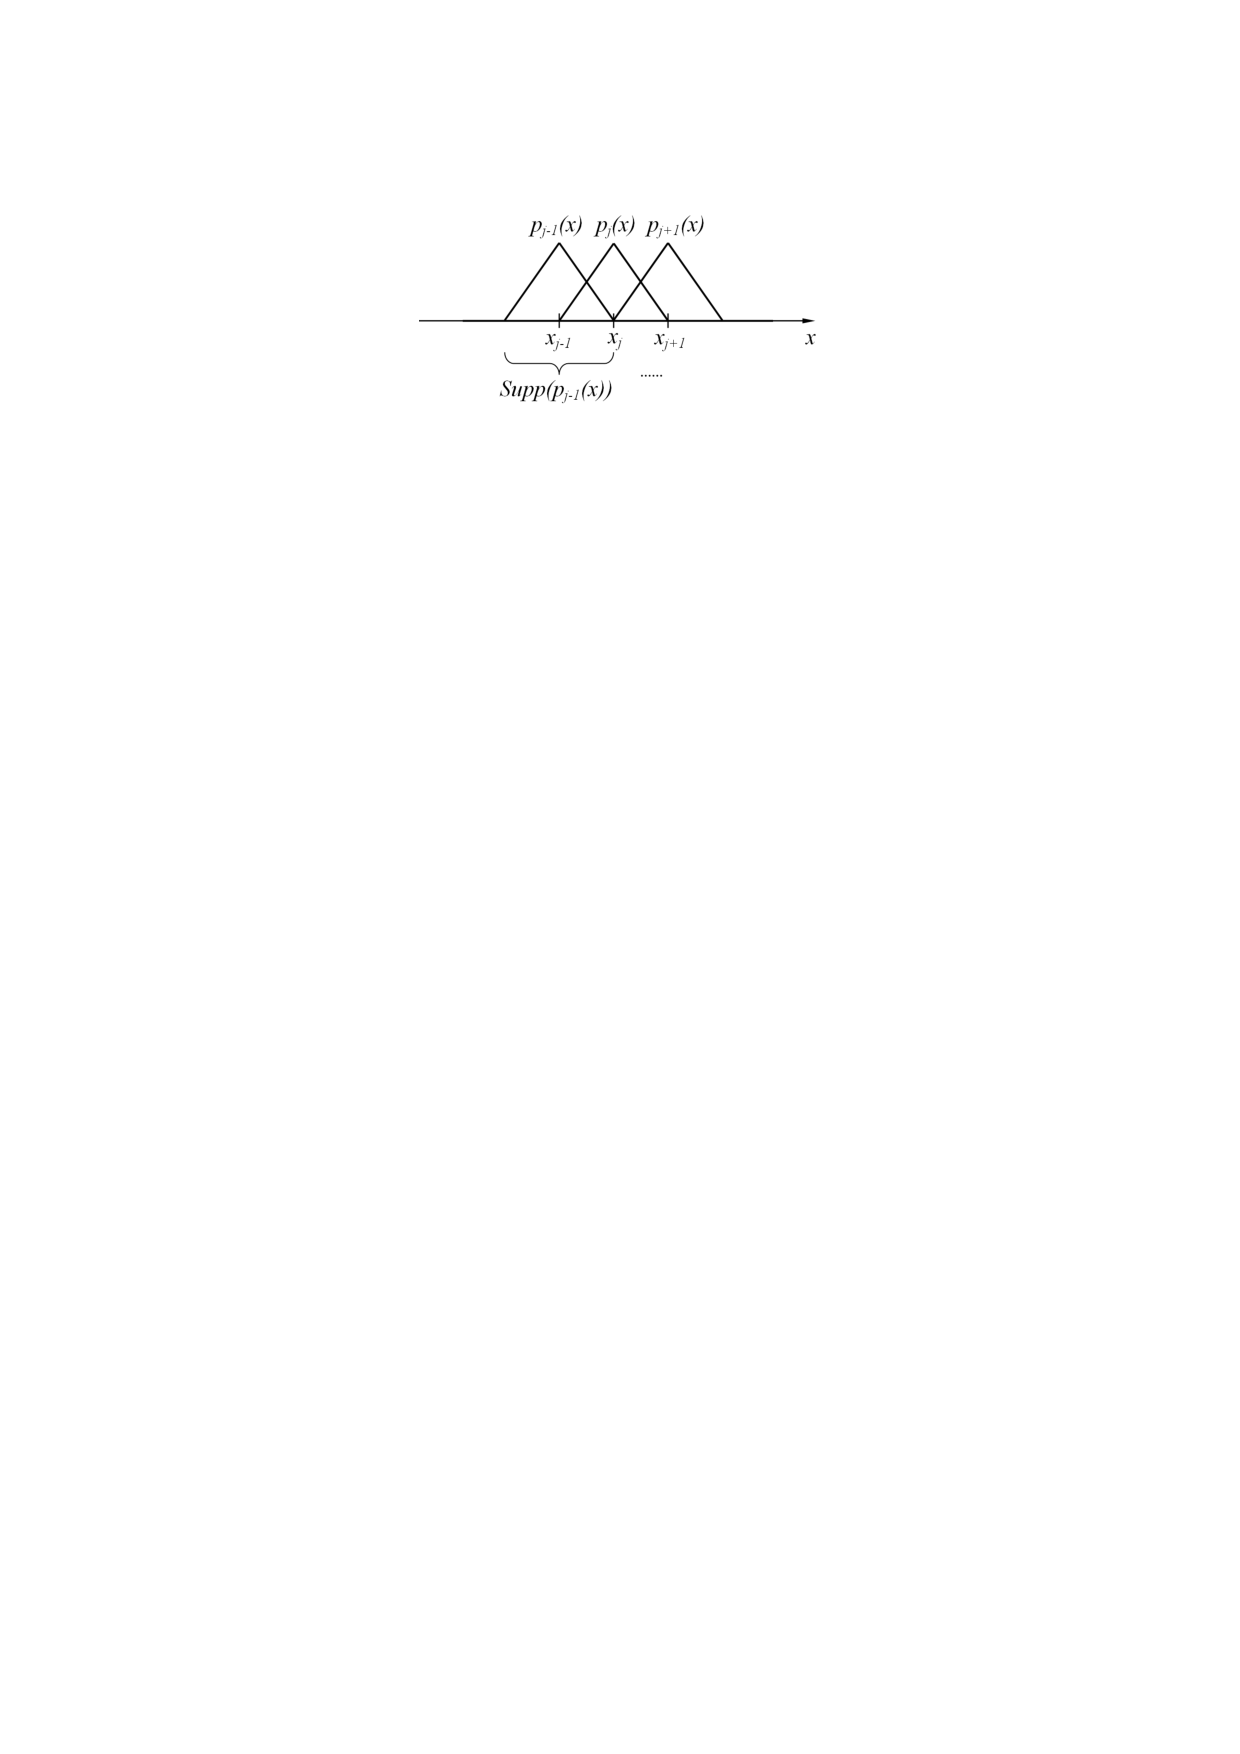
\includegraphics[width=0.7\linewidth]{img/hutfunktionen}
		\caption{Überlagerte Hutfunktionen}
		\label{fig:hutfunktionen}
	\end{figure}
	
	Damit kann das Gleichungssystem in der Form
	
	\begin{equation}
	\mathbf{S}_h \mathbf{u}_h + \mathbf{C}_h \frac{\partial}{\partial t} \mathbf{u}_h + \mathbf{M}_h \frac{\partial ^2}{\partial t^2} \mathbf{u}_h = \mathbf{0}
	\end{equation}
	
	folgendermaßen angeschrieben werden:
	
	\begin{align}
	\begin{split}
	\frac{1}{h}   
	&\begin{bmatrix}
	2 & -1 & 0 & \cdots & 0 \\ 
	-1 & 2 & -1 & \cdots & 0 \\ 
	0 & -1 & 2 & \ddots & \vdots \\ 
	\vdots & \vdots & \ddots & \ddots & -1 \\ 
	0 & 0 & \cdots & -1 & 1
	\end{bmatrix} 
	\begin{bmatrix}
	u_1 \\ 
	u_2 \\ 
	\vdots \\ 
	u_N
	\end{bmatrix}  +
	\\
	+
	\sqrt{\mu_0 \epsilon_0} 
	&\begin{bmatrix}
	0 & 0 & 0 & \cdots & 0 \\ 
	0 & 0 & 0 & \cdots & 0 \\ 
	0 & 0 & 0 & \ddots & \vdots \\ 
	\vdots & \vdots & \ddots & \ddots & 0 \\ 
	0 & 0 & \cdots & 0 & 1
	\end{bmatrix} 
	\frac{\partial}{\partial t} 
	\begin{bmatrix}
	u_1 \\ 
	u_2 \\ 
	\vdots \\ 
	u_N
	\end{bmatrix}
	+ \\ +
	\mu_0 \epsilon_0 \frac{h}{6}
	&\begin{bmatrix}
	4 & 1 & 0 & \cdots & 0 \\ 
	1 & 4 & 1 & \cdots & 0 \\ 
	0 & 1 & 4 & \ddots & \vdots \\ 
	\vdots & \vdots & \ddots & \ddots & 1 \\ 
	0 & 0 & \cdots & 1 & 2
	\end{bmatrix} 
	\frac{\partial ^2}{\partial t^2} 
	\begin{bmatrix}
	u_1 \\ 
	u_2 \\ 
	\vdots \\ 
	u_N
	\end{bmatrix} = 
	\begin{bmatrix}
	0 \\ 
	0 \\ 
	\vdots \\ 
	0
	\end{bmatrix}
	\end{split}
	\end{align}
	
	\subsection{Newmark Zeitschrittverfahren}
	
	Hier werden die partiellen Zeitableitung durch die Variablen $u, v, a$ dargestellt.
	\[
	u = u(t_j) , \quad 
	\frac{\partial u}{\partial t} \approx v(t_j) , \quad
	\frac{\partial^2 u}{\partial t^2} \approx a (t_j)
	\]
	Diese sind eine Anlehnung an die Mechanik, wo die erste Ableitung des Weges nach der Zeit die Geschwindigkeit $v$, und die zweite Ableitung nach der Zeit die Beschleunigung $a$ bezeichnet.
	Das Newmark-Verfahren beruht auf einer Taylor-Entwicklung für $u$ und $v$, wobei
zweite Ableitungen durch Beschleunigungen zum Zeitpunkt $t_j$ und $t_{j+1}$ approximiert werden. Für den Zeitpunkt $t_{j+1} = tj + \Delta t$ ergibt sich das Gleichungssystem
	
	\begin{equation}
	\mathbf{Su}_{j+1} + 	\mathbf{Cv}_{j+1} +	\mathbf{Ma}_{j+1} = 	\mathbf{f}_{j+1}
	\label{eq:newmark}
	\end{equation}
	
	\begin{align}
		v_{j+1} &= v_j + \Delta t  [(\frac{1}{2}-\gamma)a_j + \gamma a_{j+1}] \\
		u_{j+1} &= u_j + \Delta t v_j + \frac{(\Delta t)^2}{2} [(\frac{1}{2}-\beta)a_j + \beta a_{j+1}]
	\end{align}
	
	mit $\beta = \frac{1}{4}$ und $\gamma = \frac{1}{2}$.
	
	Die Gleichung \ref{eq:newmark} kann auf einen der drei Parameter umgeformt werden und es ergibt sich
	\begin{equation}
	(\mathbf{S} + \gamma \Delta t	\mathbf{C} +	\mathbf{M})a_{j+1} = 	\mathbf{\tilde f}_{j+1}
	\label{eq:newmark-final}
	\end{equation}
	wobei die Größen $u_j$, $v_j$ und $a_j$ in den Vektor $\mathbf{\tilde f}_{j+1}$ sind. Herleitung siehe Skriptum.
	
	
	\subsection{Implementierung in Matlab}
	\lstinputlisting[language=matlab,style=myMatlabStyle,caption={Implementierung der FEM für ein eindimensionales Lösen der Wellengleichung}]{../Matlab/FEM.m}	
	
	
	\subsection{Ergebnis}
	
	Die Methode der finiten Elemente in Kombination mit dem Newmark'schen Zeitschrittverfahren bringt sehr brauchbare Ergebnisse hervor. Jedoch neigt das Verfahren, trotz einhalten der Stabilitätsbedingung nach ausreichend vielen Zeitschritten
	\begin{equation}
		\Delta t < \frac{\Delta x^2}{v}
	\end{equation}
	 zur Instabilität.
	
	\begin{figure}[!h]
		\centering
		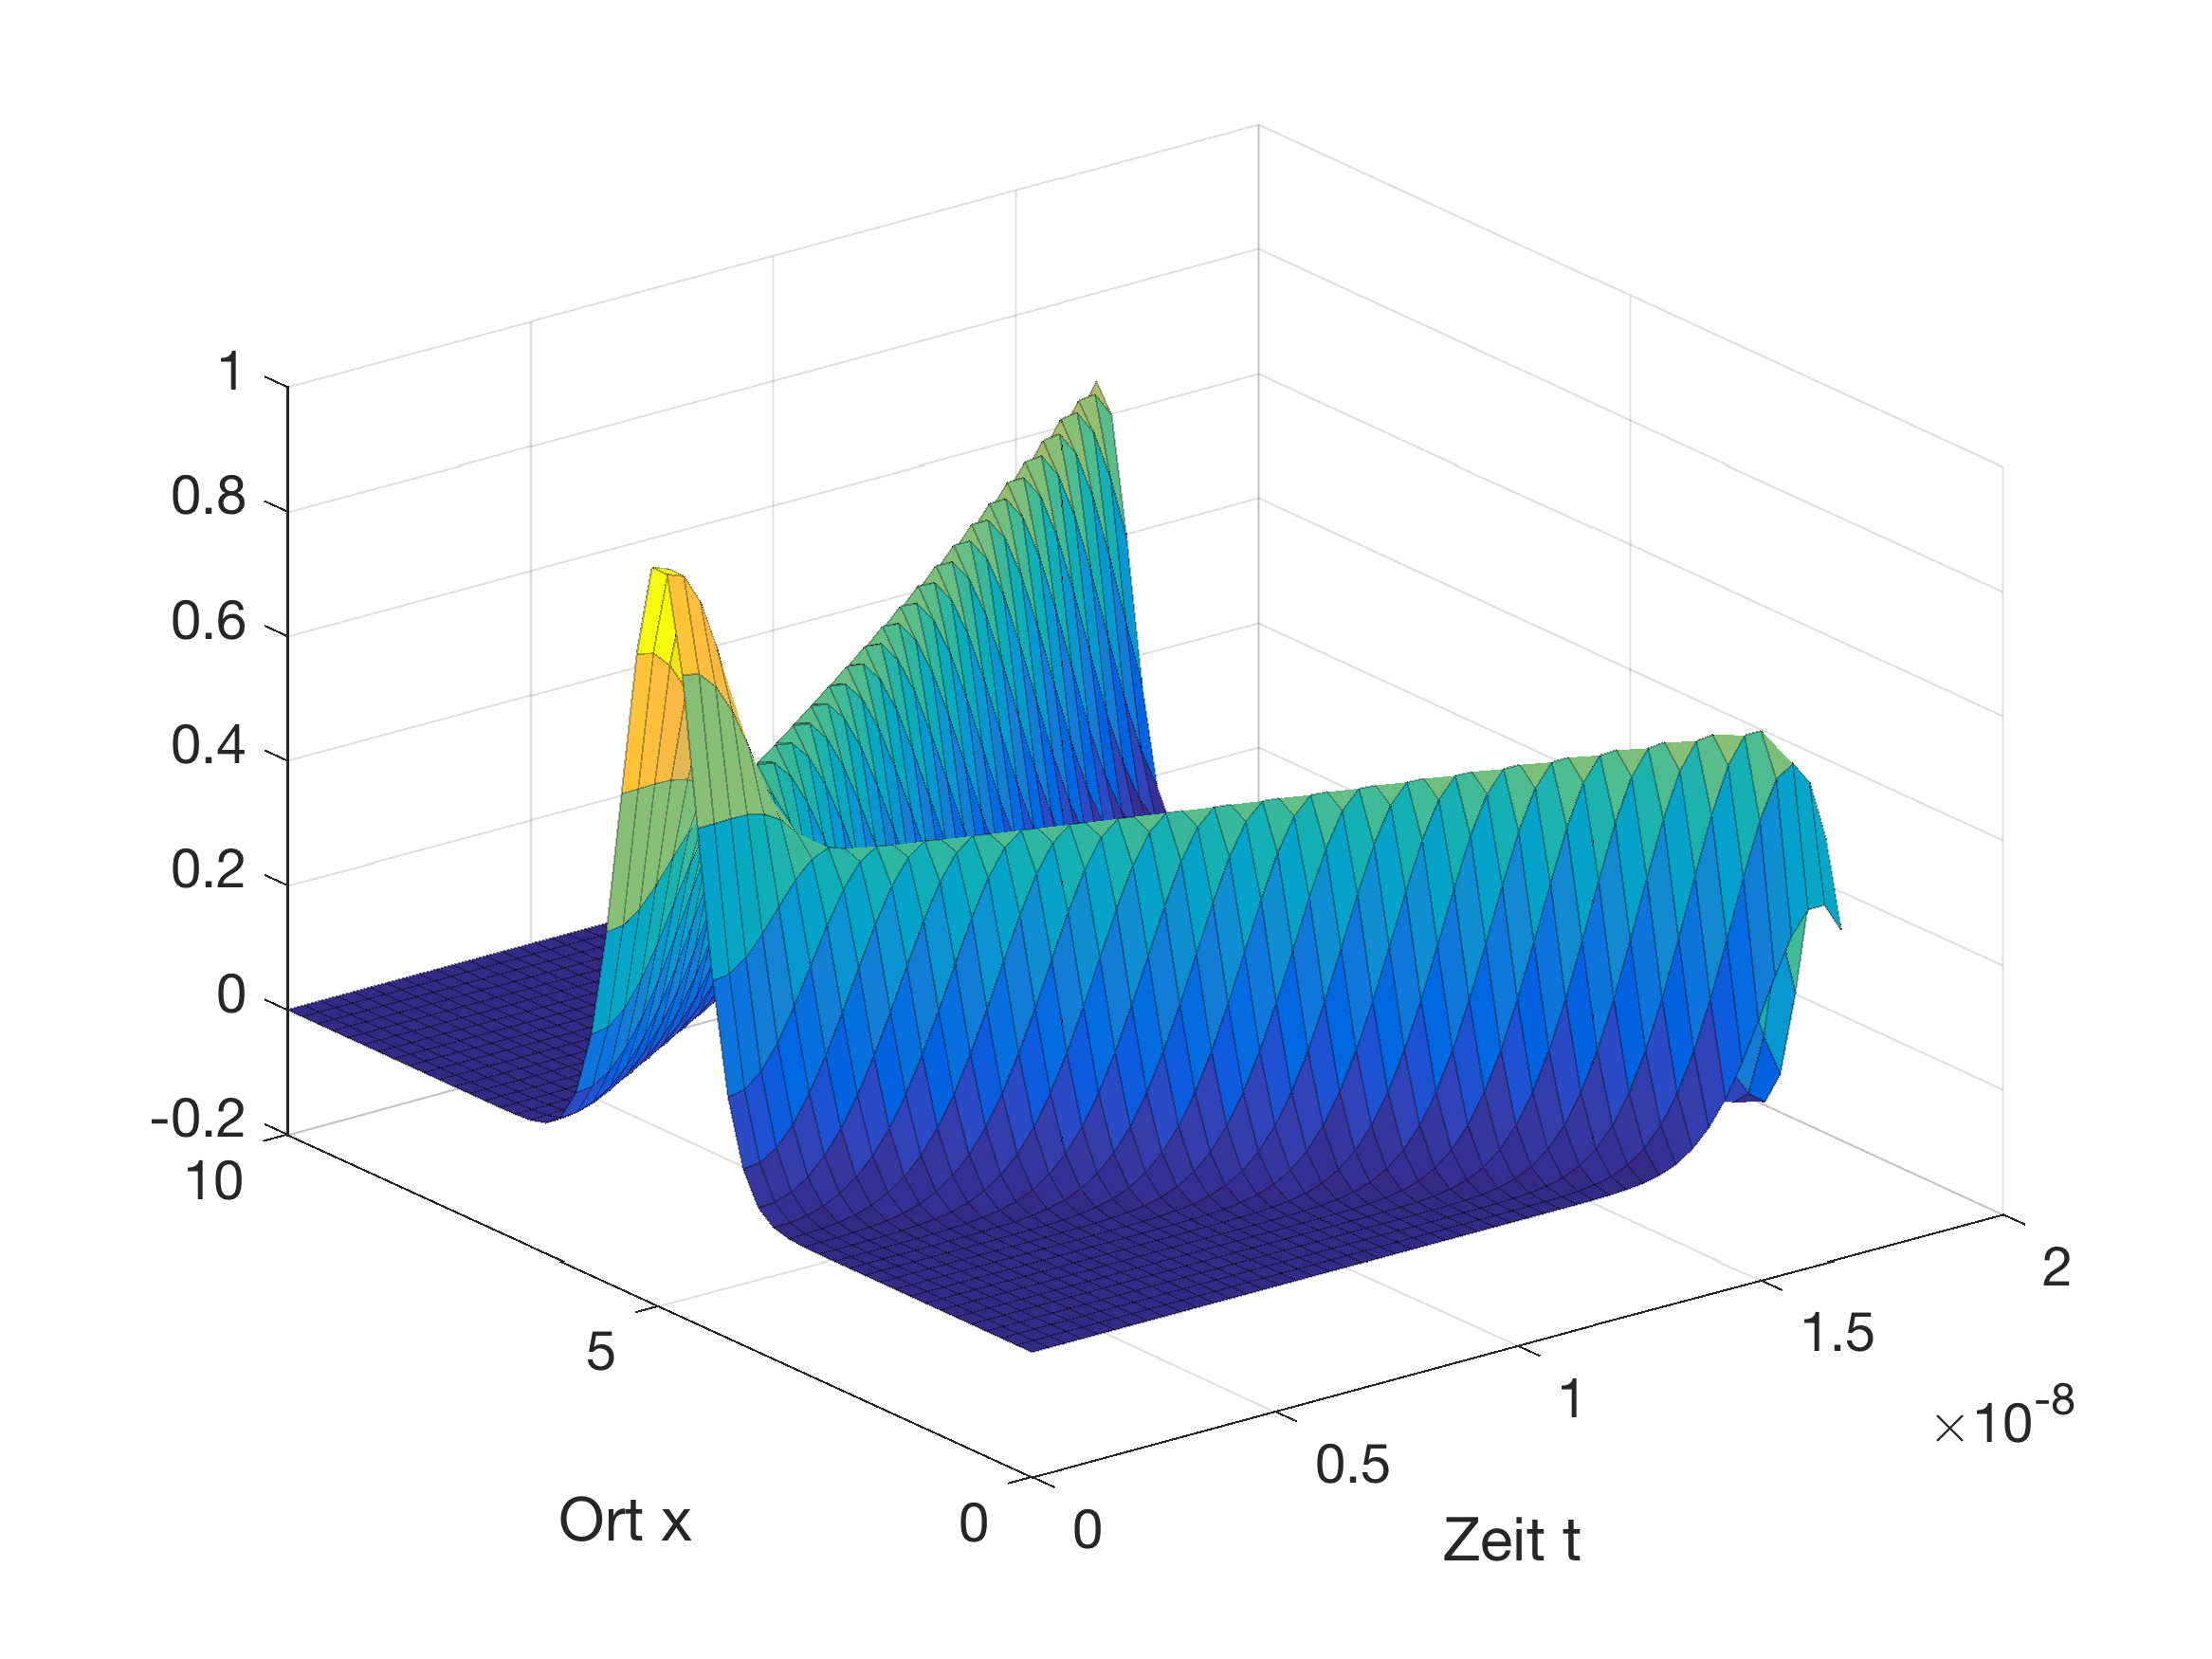
\includegraphics[width=\linewidth]{../Matlab/wave}
		\caption{Ergebnisse der FEM mit dem Newmark-Zeitschrittverfahren}
		\label{fig:wave}
	\end{figure}
	
	
	FEM Ablauf (Zusammenfassung)
	\begin{enumerate}
		\item Stelle das Gleichungssystem in der Form $Lu = f$ dar, wobei $L$ ein linearer Differentialoperator beliebiger Gestalt ist.
		\item Ersetzte deine Funktion $u$ durch $u_h$, eine gewichtete Summe von Ansatzfunktionen, mit noch zu bestimmenden Gewichten.
		\item Multipliziere die Gleichung mit einer Gewichtsfunktion $w$ und integriere über das gesamte Gebiet.
		\item Für das Galerkin-Verfahren wähle die selbe Ansatzfunktionen für $u_h$ und $w$.
		\item Löse die Integrale und stelle das Gleichungssystem in einer Matrix Schreibweise dar. Anschließend muss nur noch das lineare Gleichungssystem gelöst werden.
	\end{enumerate}